% STRATIA -- CVPR 2027 submission draft. Build: pdflatex main; bibtex main; pdflatex main; pdflatex main.
% Every number in the prose comes from numbers.tex and every table from tables/*.tex, both generated by
% scripts/reproduce_tables.py from the committed result files (results/P090_locked_test.json, data/*.parquet).

\documentclass[10pt,twocolumn,letterpaper]{article}

%%%%%%%%% PAPER TYPE  - PLEASE UPDATE FOR FINAL VERSION
% \usepackage{cvpr}              % To produce the CAMERA-READY version
\usepackage[review]{cvpr}      % To produce the REVIEW version
% \usepackage[pagenumbers]{cvpr} % To force page numbers, e.g. for an arXiv version

%% This file contains a number of tweaks that are typically applied to the main document.
%% They are not enabled by default, but can be enabled by uncommenting the relevant lines.


%%
%% Official support for 2-column teaser figure
%%
\usepackage{cuted} %< for strip environment

%%
%% For auto-referencing of figures (see fig/teaser.tex and \label{} therein) 
%%
\usepackage{currfile} %< for \currfilebase macro

%%
%% caption and (global) spacing overrides
%%
\usepackage{caption} %< for "\captionof" commands (teaser)
% \setlength{\abovecaptionskip}{.5em} % space above caption
% \setlength{\belowcaptionskip}{1em} % space below caption

%%
%% Inline annotations; for predefined colors, refer to "dvipsnames" in the xcolor package:
%% https://tinyurl.com/overleaf-colors
%%
\newcommand{\red}[1]{{\color{red}#1}}
\newcommand{\todo}[1]{{\color{red}#1}}
\newcommand{\TODO}[1]{\textbf{\color{red}[TODO: #1]}}
%%
%% Disable for camera ready / submission by uncommenting these lines:
%%
% \renewcommand{\TODO}[1]{}
% \renewcommand{\todo}[1]{#1}

%%
%% Work harder in optimizing text layout. Typically shrinks text by 1/6 of page, enable
%% it at the very end of the writing process, when you are just above the page limit.
%%
% \usepackage{microtype}

%%
%% Fine-tune paragraph spacing.
%%
% \renewcommand{\paragraph}[1]{\vspace{.5em}\noindent\textbf{#1.}}

%%
%% Globally adjusts space between figure and caption.
%%
% \setlength{\abovecaptionskip}{.5em}

%%
%% Allows "the use of \paper to refer to the project name"
%% with automatic management of space at the end of the word.
%%
% \usepackage{xspace}
% \newcommand{\paper}{ProjectName\xspace}

%%
%% Commonly used math definitions.
%%
% \DeclareMathOperator*{\argmin}{arg\,min}
% \DeclareMathOperator*{\argmax}{arg\,max}

%%
%% Tighten underline.
%%
% \usepackage{soul}
% \setuldepth{foobar}

%%
%% Reconfigure paragraph (tweaks spacing)
%%

% generated by scripts/reproduce_tables.py from the committed result files; do not edit
\newcommand{\nLodoModel}{0.540}
\newcommand{\nLodoProbe}{0.529}
\newcommand{\nIndGenusModel}{0.706}
\newcommand{\nIndGenusProbe}{0.733}
\newcommand{\nCtwoEtage}{0.93}
\newcommand{\nCtwoOktas}{0.96}
\newcommand{\nSkillOldlr}{0.54}
\newcommand{\nSkillWeste}{0.44}
\newcommand{\nMaeModel}{872}
\newcommand{\nMaeRidge}{1096}
\newcommand{\nCovEighty}{0.72}
\newcommand{\nMaeClim}{2012}
\newcommand{\nSkillAll}{0.57}
\newcommand{\nCovNinetyFive}{0.92}
\newcommand{\nCovRaw}{0.88}
\newcommand{\nSkyMiou}{0.900}
\newcommand{\nLayerMiou}{0.668}
\newcommand{\nOodAuroc}{0.94}
\newcommand{\nZsEtage}{0.00}
\newcommand{\nZsOktas}{0.02}
\newcommand{\nZsOod}{0.51}
\newcommand{\nAdEtage}{0.46}
\newcommand{\nAdOktas}{0.67}
\newcommand{\nAdGenus}{1.00}
\newcommand{\nClearCloud}{0.28}
\newcommand{\nAlphaEtageHumans}{0.659}
\newcommand{\nAlphaEtageModel}{0.684}
\newcommand{\nLooEtageModel}{0.932}
\newcommand{\nLooEtageHumans}{0.893}
\newcommand{\nLooOktasModel}{0.892}
\newcommand{\nLooOktasHumans}{0.909}
\newcommand{\nParamsM}{23.4}
\newcommand{\nHeadsParamsM}{1.76}
\newcommand{\nGFlops}{46}
\newcommand{\nLatencyGpu}{20}
\newcommand{\nLatencyCpu}{144}
\newcommand{\nLatencyDml}{29}
\newcommand{\nAblNoGeo}{0.809}
\newcommand{\nAblGeoAlways}{0.829}
\newcommand{\nAblHard}{0.794}
\newcommand{\nAblNoH}{0.813}
\newcommand{\nAblKendall}{0.814}
\newcommand{\nAblRef}{0.817}


\definecolor{cvprblue}{rgb}{0.21,0.49,0.74}
\usepackage[pagebackref,breaklinks,colorlinks,allcolors=cvprblue]{hyperref}

\def\confName{CVPR}
\def\confYear{2027}

\title{STRATIA: Honest Cloud Understanding from a Single Sky Camera\\
with Geometry-Aware Heads, Locked Tests and a Human Ceiling}

\author{Anonymous \confName~submission\\
}

\begin{document}
\maketitle
\begin{abstract}
Ground-based sky cameras are cheap, but the models trained on them are usually evaluated on leaked splits, forced
single labels and one camera. We present STRATIA, a single-image model that reads cloud genus, \'etage, cover in
oktas, a per-pixel sky parse and a calibrated cloud-base height (CBH) distribution from one all-sky picture, and
the protocol that makes its numbers believable. A leakage audit of 52,425 images from seven public datasets and our
own camera removes duplicate and same-scene images from across splits, harmonises the labels into the WMO
genus/\'etage hierarchy as \emph{sets}, and measures a human ceiling from five expert annotators. The model keeps a
frozen DINOv3 ViT-S/16 backbone and adds a \emph{SkyRay} encoder that tells each token where in the sky it looks
(a ray map from the camera calibration and the Sun's position), with geometry dropout so unknown geometry is a valid
input. Success criteria were pre-registered and the test sets locked and read once. On them, the model reaches
\nCtwoEtage{} of expert--expert agreement on \'etage sets and \nCtwoOktas{} on cover; as a sixth annotator it ranks
second of six on \'etage sets. Its cloud-base height, learned from ceilometer-paired frames of a camera network,
has skill \nSkillOldlr{} over climatology at a seen site and \nSkillWeste{} at a site never seen in training,
\nMaeModel{}\,m MAE against \nMaeRidge{}\,m for a ridge on the same frozen features. Two pre-registered claims
fail and we report them: cross-dataset \'etage transfer does not beat a linear probe (\nLodoModel{} vs
\nLodoProbe{} macro-F1), and split-conformal intervals fitted on spring weeks cover \nCovEighty{} instead of 0.80 on a
different season. The deployed graph runs at \nLatencyDml{}\,ms per frame on a laptop GPU inside an open desktop
application, flags out-of-distribution skies (AUROC \nOodAuroc{}), and adapts to a new camera from three afternoons
of captures. Code, splits, data card and the locked results are released.
\end{abstract}

\section{Introduction}
\label{sec:intro}

Knowing what the sky is doing above a point still takes a trained observer or a ceilometer. An observer reports
cloud genus, amount and base height by eye following the WMO conventions~\cite{wmo2017atlas}; a ceilometer
measures the base height along one vertical line and costs more than most of the stations that would like one.
Upward-looking cameras cost a few thousand rupees, and a decade of work has shown that cloud type, cover and even
base height can be read from their pictures~\cite{zhang2018cloudnet,dev2017colorbased,liu2020mgcd}. Yet almost
none of that work transfers to a camera it was not trained on, and much of it reports numbers that do not survive
a second look.

Three problems stand between the published results and a deployable model. First, \emph{leakage}: the popular
recognition sets are built from web images and time series; exact and near-duplicate images straddle train and
test splits, and the same scene appears minutes apart. Our audit (\cref{sec:data}) finds that the 91--97\,\%
accuracies reported on CCSN~\cite{zhang2018cloudnet} fall to 57--62\,\% once duplicates are grouped. Second,
\emph{forced labels}: experts disagree on cloud type on a large fraction of images; a single hard label hides a
measurable ceiling, and a model scored against it is scored against noise. Third, \emph{one camera}: a classifier
that has never seen another lens, exposure or horizon does not know that it is looking at a new sky; it answers
anyway.

This paper treats those three problems as the method. We assemble seven public datasets and our own camera into a
single corpus with grouped, day-blocked and leave-one-dataset-out splits, WMO-harmonised \emph{set-valued} labels
and a human ceiling measured from five annotators; we pre-register the success criteria and lock the test sets
before any model is trained, and read them once. On that footing we build STRATIA (\cref{fig:teaser}): a frozen
DINOv3 ViT-S/16 backbone~\cite{simeoni2025dinov3}, a \emph{SkyRay} encoder that adds to every token the direction it
looks at (from the camera calibration) and where the Sun is, with geometry dropout so that ``unknown'' geometry is a
valid input, and heads for genus and \'etage sets, ordinal cover, a sky/cloud/glare parse with cloud layers, an
ordinal cloud-base height distribution supervised by ceilometers of an all-sky camera network~\cite{eye2sky}, and
an out-of-distribution score that turns into an explicit \emph{uncertain} state. The whole model exports to one ONNX
graph with its calibration folded in, and runs inside an open desktop application on a laptop GPU.

\paragraph{Contributions.}
\begin{itemize}
\item A leakage-audited, WMO-harmonised benchmark protocol for sky cameras: grouped and temporal splits, LODO
  folds, a held-out station, set-valued labels, a measured expert ceiling, and locked test sets with a logged
  single read (\cref{sec:data}).
\item STRATIA: geometry-aware heads on a frozen foundation backbone, trained on cached features in stages, with
  temperature and split-conformal calibration and an OOD score (\cref{sec:method}).
\item Locked-test results with bootstrap intervals (\cref{sec:experiments}): expert-level agreement on
  \'etage and cover, ceilometer-level cloud-base height that transfers to a site never seen in training, and two
  pre-registered negatives reported as such.
\item A few-shot adaptation to the authors' own camera from three afternoons, verified on a locked fourth day, and
  a working deployment (\cref{sec:b0268}).
\end{itemize}

\section{Related Work}
\label{sec:related}

\paragraph{Ground-based cloud classification.} CCSN~\cite{zhang2018cloudnet} introduced an eleven-class genus set
of web images and a CNN baseline; the Tianjin multimodal series (MGCD)~\cite{liu2020mgcd} added a camera and
weather variables; SWIMCAT~\cite{dev2017colorbased} groups five sky types. Reported accuracies are high but the
protocols are random image splits; our audit (\cref{sec:data}) and that of others on near-duplicate web
data~\cite{barz2020duplicates} show why such numbers do not transfer. We keep the datasets and change the protocol.

\paragraph{Sky parsing and layers.} Colour-based and learned segmentation of sky versus cloud is well studied on the
SWIMSEG/SWINSEG family~\cite{dev2017colorbased}; multi-layer masks exist for one all-sky camera set in
Almer\'ia~\cite{almeria2025}. We train one dense head for both on frozen tokens with a light DPT-style
decoder~\cite{ranftl2021dpt}.

\paragraph{Cloud-base height from cameras.} Stereo pairs of all-sky imagers and ceilometer references give
base heights for a network~\cite{blum2021cloudheight,eye2sky}; single-camera height from appearance alone is rarer and rarely
calibrated. We learn a 24-bin ordinal height distribution from ceilometer-paired frames and report it with
split-conformal intervals~\cite{vovk2022conformal,angelopoulos2023conformal}.

\paragraph{Expert disagreement as a ceiling.} Krippendorff's alpha~\cite{krippendorff2004content} and
leave-one-out agreement are standard in annotation studies; the Montenegro expert set~\cite{montenegro2025}
provides five raters per image and lets us put a model on the same footing as a human annotator rather than
against a majority vote.

\paragraph{Foundation features and the sky.} Self-supervised ViTs transfer as frozen feature
extractors~\cite{simeoni2025dinov3,oquab2024dinov2}; linear probes on them are strong baselines for recognition,
which is why our pre-registered transfer criterion is measured against the best such probe. Geometry-conditioned
tokens are common in 3D vision; feeding the ray direction of every patch, with the Sun, to a sky model is, to our
knowledge, new.

\paragraph{Calibration and OOD.} Temperature scaling~\cite{guo2017calibration}, Mahalanobis~\cite{lee2018mahalanobis}
and energy~\cite{liu2020energy} scores are the components we combine; we fit all of them on validation data and
test them once.

\section{Data and Protocol}
\label{sec:data}

\paragraph{Sources.} Seven public datasets and our own camera: CCSN~\cite{zhang2018cloudnet} (2,543 web images,
11 genera with alternatives), MGCD~\cite{liu2020mgcd} (8,000 camera images, 7 sky types), SWIMCAT and the
SWIMSEG/SWINSEG/SWINySEG family~\cite{dev2017colorbased} (sky types and sky/cloud masks), Montenegro~\cite{montenegro2025}
(2,522 all-sky images with five expert annotations each: altitude class, genus codes, cover in oktas),
Almer\'ia~\cite{almeria2025} (818 all-sky images with sky/cloud/layer masks), Eye2Sky~\cite{eye2sky} (four all-sky
imagers with CHM15k ceilometers at two of them; April--July 2022), and B0268, a 16-megapixel fisheye camera on
the authors' rooftop in Bengaluru (393 labelled frames over four afternoons). The corpus holds 52,425 images; the
data card lists every licence.

\paragraph{Leakage audit.} Perceptual hashes under the dihedral group, DINOv3 embeddings and the datasets' own
metadata find 661 exact duplicates in 312 within-dataset groups, 34.6\,\% of SWINySEG as flipped or rotated copies
of SWIMSEG/SWINSEG, MGCD's 8,000 images in about 227 same-scene groups, and CCSN images that carry a second genus
on a copy of themselves (7.9\,\%). Temporal autocorrelation puts Eye2Sky frames of one day at 82--92\,\% same-scene
similarity, decorrelating only across days; Montenegro is correlated across days and needs contiguous blocks of at
least seven days. A shortcut audit shows that dataset identity is readable from frozen features at 99.7\,\% and
the Eye2Sky station at 100\,\%: camera identity cannot be masked, so the protocol holds out cameras and datasets
rather than images. The CCSN number that motivates all of this: a grouped split scores \emph{lower} than the random
split (0.511 vs 0.588 macro-F1 for the same probe), because the random split's errors are concentrated on the
duplicates that leaked.

\paragraph{Harmonisation.} Every native label maps into the WMO hierarchy (genus $\rightarrow$ \'etage) as a
\emph{set}: a CCSN image with an alternative genus keeps both, a Montenegro image keeps the share of raters per
genus and \'etage and the distribution of oktas, an Eye2Sky frame paired with a ceilometer gets the \'etage of the
lowest base as a known positive and the \'etages below it as weak negatives. Losses are masked where a label is
unknown. The human ceiling on Montenegro is the leave-one-out agreement of a rater with the majority of the
others: 0.852 on the \'etage set and 0.873 on cover within $\pm1$ okta (alpha 0.66 and 0.96).

\paragraph{Splits and the lock.} In-domain splits assign whole duplicate or temporal \emph{units} to train, val
and test (70/10/20) with conflicting images never in test; leave-one-dataset-out (LODO) folds hold out a whole
source; a held-out-station split holds out one Eye2Sky camera; the ceilometer pairs are split by day with the second
site's data entirely in test for one model; the B0268 frames are split by day with the last day locked. The 23 test
manifests are hashed into a lock file that CI checks; the research design fixed three success criteria on
validation data before training (C1 transfer, C2 expert agreement, C3 cloud-base height); the locked sets were
read once, with the reason logged, and every number from them in this paper comes from that one read.

\section{Method}
\label{sec:method}

\begin{figure*}[t]
\centering
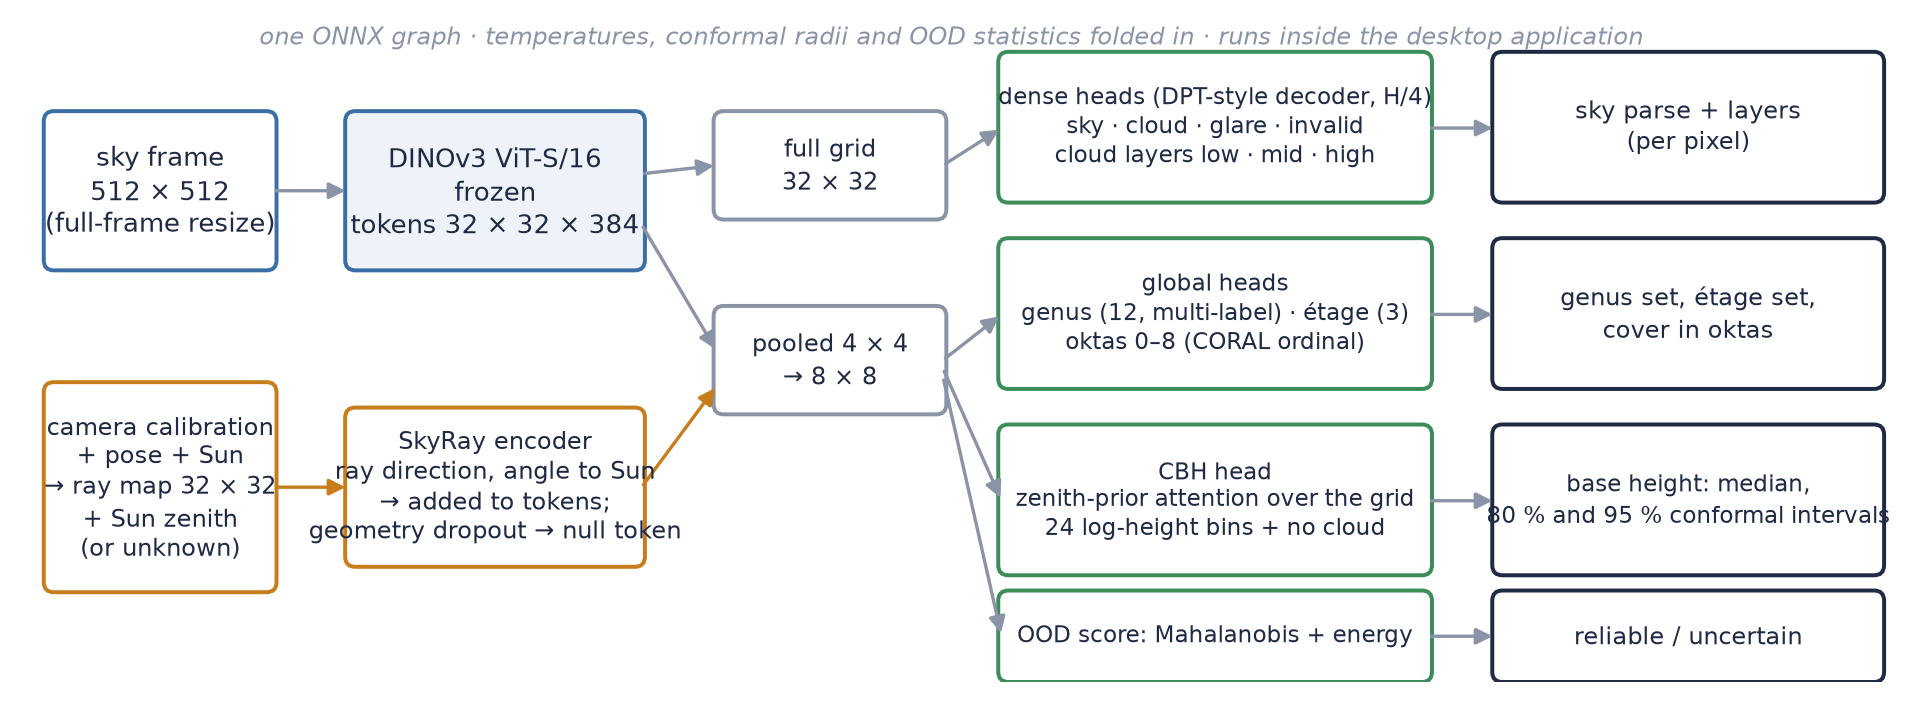
\includegraphics[width=0.98\textwidth]{fig/architecture.png}
\caption{STRATIA. A frozen DINOv3 ViT-S/16 turns the 512$\times$512 frame into 32$\times$32 tokens. The
\emph{SkyRay} encoder adds to each pooled token the unit direction it looks at (ray map from the camera calibration)
and the Sun's position, or a learned null token when geometry is unknown. Global heads read genus, \'etage and
ordinal cover; dense heads parse sky, cloud and glare and the cloud layers; the CBH head reads an ordinal height
distribution over 24 log-spaced bins; a Mahalanobis+energy score gives the reliability. The graph is exported with
its calibration folded in and runs in the desktop application.}
\label{fig:teaser}
\end{figure*}

\paragraph{Backbone and geometry.} The image is resized full-frame to 512$\times$512 (no crop, no mask zeroing) and
encoded by a frozen DINOv3 ViT-S/16~\cite{simeoni2025dinov3}; the global and CBH heads work on the token grid
average-pooled to 8$\times$8, the dense heads on the full 32$\times$32 grid. The ray map gives, for every patch, the
unit direction of its centre in a world frame from the camera's fisheye or pinhole calibration and pose (validated
against the Sun's track, median error 0.1$^\circ$ on the Eye2Sky stations), plus a validity flag; the metadata
vector carries the Sun's zenith angle. The SkyRay encoder projects the ray direction and the angle to the Sun into
the token dimension and adds them; with probability $p$ during training (and whenever a host has no calibration)
the geometry is replaced by a learned null token, so a frame from an unknown camera is a valid input rather than a
corrupted one.

\paragraph{Heads and losses.} Genus is a 12-way multi-label head (ten genera, clear, contrail) with a masked BCE
against set-valued or soft targets; \'etage is a three-way multi-label head tied to the genera by a hierarchy loss
($\lambda_h=0.1$) that penalises an \'etage without a genus in it; cover is a CORAL ordinal head over 0--8 oktas
trained on rater distributions. The dense heads are a two-stage DPT-style decoder at $H/4$ with 1$\times$1 heads for
the four sky-parse classes and three layers, cross-entropy with ignore labels. The CBH head attends over the grid
with a zenith-aligned prior from the ray map and predicts a 24-bin log-height distribution plus a no-cloud bin,
trained with a Gaussian soft target in log height and a CRPS term; the median of the distribution is the point
estimate. The OOD score standardises an energy term on the genus logits and a Mahalanobis distance of the pooled
feature to the training distribution; its threshold is the 95th percentile of in-domain validation scores.

\paragraph{Training.} Heads train on cached backbone features in three stages (global, dense, CBH) with a
task-balanced sampler across sources, AdamW, cosine schedule, EMA weights and early stopping on the mean \'etage
macro-F1 over sources; joint multi-task training and LoRA unfreezing of the last blocks were tried and are reported
as ablations. All selection uses validation units.

\paragraph{Calibration.} A temperature per head is fitted on validation rows (genus by ECE, the others by NLL; the
\'etage and cover temperatures stay at 1), the CBH head's 80\,\% and 95\,\% intervals are split-conformal radii in
CDF units fitted on the validation days, and the OOD threshold is fixed as above. All of it is folded into the
exported ONNX graph (opset 17; PyTorch--ONNX Runtime parity $\le 1.6\times10^{-4}$), so the deployed and the reported
model are one object.

\paragraph{Adapting to a new camera.} For the authors' camera the global heads are fine-tuned on cached features
of the labelled afternoons with 16$\times$ replay of the source data and a regression guard (no mean \'etage or genus
F1 drop of more than 0.02 on the source validation split; one of six draws exceeded it by 0.01 and is recorded);
the backbone stays frozen and the dense and CBH heads are untouched. The calibration is refitted and the graph
re-exported as a new version.

\section{Experiments}
\label{sec:experiments}

All test numbers in this section come from one logged read of the locked test sets (\cref{sec:data}); every
other number is on validation units. Intervals are 95\,\% cluster bootstraps over the split units (duplicate or
temporal groups, days for the ceilometer pairs), 1,000 resamples. Baselines are a linear probe on the best frozen
backbone of our own probe sweep (DINOv3 ViT-L/16 for in-domain genus, ViT-B/16 for cross-dataset \'etage) and a
ridge on the same frozen features for cloud-base height, so that every comparison isolates what the heads add.

\subsection{Pre-registered criteria}
\begin{table}[t]
\centering
\small
\begin{tabular}{llrlrll}
\toprule
 & Quantity & Val & Test [95\% CI] & Reference & Required & Holds \\
\midrule
C1 & LODO étage macro-F1, mean of the four folds & 0.548 & 0.540 & 0.529 & $\geq$ reference + 0.05 & no \\
C1 & in-domain genus macro-F1 (CCSN, MGCD) & 0.719 & 0.706 & 0.733 & $\geq$ reference $-$ 0.01 & no \\
C2 & Montenegro étage-set agreement / human ceiling & 1.047 & 0.926 & 0.900 & $\geq$ 0.90 & yes \\
C2 & Montenegro oktas $\pm$1 agreement / human ceiling & 1.027 & 0.963 & 0.900 & $\geq$ 0.90 & yes \\
C3 & CBH skill, OLDLR (CDLRA) pairs & 0.471 & 0.536 [0.440, 0.630] & 0.200 & $\geq$ 0.20 & yes \\
C3 & CBH skill, WESTE (CDLRB) pairs, OLDLR-only training & 0.448 & 0.436 [0.276, 0.585] & 0.100 & $\geq$ 0.10 & yes \\
C3 & CBH MAE (m), all pairs, against the frozen-feature ridge & 566 & 872 [679, 1055] & 1096 & $\leq$ 0.9 $\times$ reference & yes \\
C3 & 80 \% interval coverage with the P089 temperature and radius & 0.802 & 0.720 & 0.800 & 0.75–0.85 & no \\
\bottomrule
\end{tabular}
\caption{Pre-registered criteria on validation (Gate G4) and on the locked test sets, read once.}
\label{tab:criteria}
\end{table}

\Cref{tab:criteria} is the paper in one table. The three criteria were fixed before training with their
thresholds; two of the eight clauses fail on the test read and we leave them failed. C1 asked the heads to beat the
probe on cross-dataset \'etage by 0.05 macro-F1 and to match it within 0.01 on in-domain genus; the heads lead the
probe by \nLodoModel{} to \nLodoProbe{} (within the interval) and trail the larger ViT-L probe on genus
(\nIndGenusModel{} vs \nIndGenusProbe{}). C2 asked for 90\,\% of the expert ceiling on the five-rater set and holds
on both \'etage sets (\nCtwoEtage{}) and cover (\nCtwoOktas{}). C3 asked for skill over climatology at the seen site
and at a site never trained on, and for a 10\,\% MAE lead over the ridge; all three hold with the test intervals
clear of the thresholds. Its fourth clause, 80\,\% conformal coverage, does not: the intervals fitted on the spring
validation days cover \nCovEighty{} of the summer test pairs, where the climatology MAE itself grows from 1,147\,m
to \nMaeClim{}\,m. The calibration transfers worse than the point estimate.

\subsection{Recognition}
\begin{table*}[t]
\centering
\footnotesize
\begin{tabular}{llrr}
\toprule
Protocol & Source & STRATIA & Linear probe \\
\midrule
in-domain genus & CCSN & 0.591 [0.54, 0.63] & 0.549 [0.50, 0.59] \\
in-domain genus & MGCD & 0.821 [0.71, 1.00] & 0.918 [0.76, 0.95] \\
in-domain étage & ccsn & 0.719 [0.68, 0.76] & – \\
in-domain étage & mgcd & 1.000 [1.00, 1.00] & – \\
in-domain étage & montenegro & 0.680 [0.63, 0.72] & – \\
in-domain étage & almeria & 0.803 [0.68, 0.86] & – \\
LODO étage (held out) & ccsn & 0.451 [0.43, 0.47] & 0.396 [0.38, 0.41] \\
LODO étage (held out) & mgcd & 0.709 [0.62, 0.78] & 0.860 [0.79, 0.92] \\
LODO étage (held out) & montenegro & 0.367 [0.30, 0.45] & 0.463 [0.39, 0.53] \\
LODO étage (held out) & almeria & 0.634 [0.60, 0.66] & 0.397 [0.36, 0.43] \\
\bottomrule
\end{tabular}
\caption{Recognition on the locked test sets: STRATIA against the strongest linear probe of Stage F (ViT-L/16 for in-domain genus, ViT-B/16 for LODO étage), macro-F1 with cluster-bootstrap 95\% intervals.}
\label{tab:recognition}
\end{table*}

\Cref{tab:recognition} breaks the criteria down by source. The heads win where the probe has the least to go on
(CCSN genus with its alternatives, Almer\'ia and CCSN \'etage held out) and lose on MGCD, whose seven sky types a
linear probe already separates at 0.918, and on Montenegro held out, where the mid \'etage is rare (2\,\% of
images) and the heads over-predict ``high''. The error analysis (\cref{fig:confusion}) shows where the remaining
genus errors live: stratus and stratocumulus are swapped on 18.5\,\% of their CCSN rows, cirrus and cirrostratus
on 7.0\,\%, altostratus and nimbostratus on 6.4\,\%, and MGCD altocumulus is read as stratocumulus 71\,\% of the
time, pairs that human annotators also split on. The mid \'etage is the one the model misses most, on every source
that has it (35--46\,\% missed at the 0.5 threshold).

\begin{figure}[t]
\centering
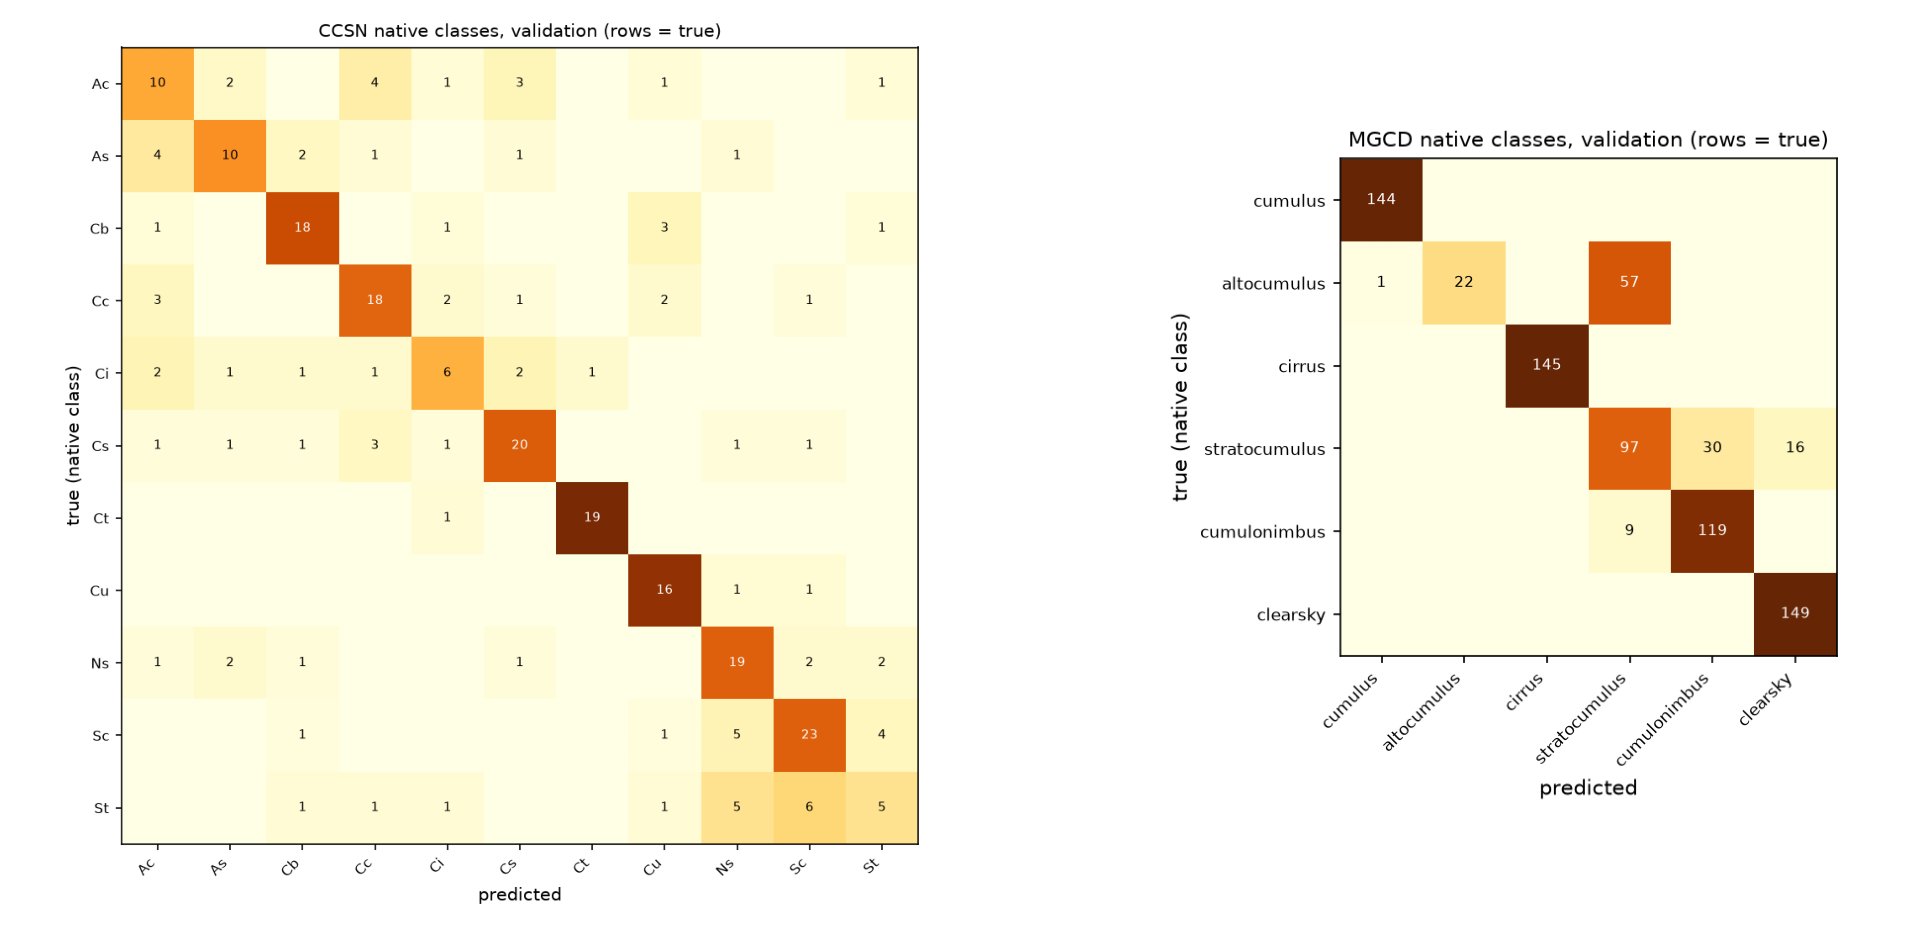
\includegraphics[width=\linewidth]{fig/genus_confusion.png}
\caption{Genus confusion on validation, native classes, for CCSN (left) and MGCD (right). Errors concentrate on
the pairs that the WMO hierarchy itself places as neighbours.}
\label{fig:confusion}
\end{figure}

\subsection{Against the expert ceiling}
\begin{table*}[t]
\centering
\footnotesize
\begin{tabular}{lrrrr}
\toprule
Quantity & Alpha (humans) & Alpha (+ model) & Model vs others & Human vs others \\
\midrule
étage set & 0.659 & 0.684 & 0.932 & 0.893 \\
oktas 0-8 & 0.960 & 0.956 & 0.892 & 0.909 \\
\bottomrule
\end{tabular}
\caption{STRATIA as a sixth Montenegro annotator (validation images): Krippendorff's alpha without and with the model, and agreement with the majority of the other raters.}
\label{tab:humanceiling}
\end{table*}

C2 compares with the ceiling as a ratio; \cref{tab:humanceiling} puts the model in the annotators' seats. Adding
STRATIA as a sixth rater raises Krippendorff's alpha on \'etage sets from \nAlphaEtageHumans{} to
\nAlphaEtageModel{} (the model agrees with the group more than the average human does) and leaves cover alpha
unchanged within 0.004. In leave-one-out terms the model agrees with the other raters' majority on
\nLooEtageModel{} of images against a human mean of \nLooEtageHumans{}, which ranks it second of six raters; on
cover it ranks last of six, at \nLooOktasModel{} against \nLooOktasHumans{}, close behind the humans. These are
validation images (the Montenegro test set is two blocks of days and too small to rank six raters).

\subsection{Cloud-base height}
\begin{table*}[t]
\centering
\footnotesize
\begin{tabular}{lrrrr}
\toprule
Model & MAE (m) [CI] & Skill [CI] & $\pm$500 m & 80\% cov. \\
\midrule
STRATIA (both sites in training) & 872 [679, 1055] & 0.566 [0.48, 0.66] & 0.546 & 0.720 \\
  OLDLR (CDLRA) & 933 [744, 1127] & 0.536 [0.44, 0.63] & 0.531 & 0.698 \\
  WESTE (CDLRB) & 813 [601, 1013] & 0.596 [0.50, 0.70] & 0.561 & 0.742 \\
STRATIA, geometry zeroed & 875 [680, 1050] & 0.565 [0.48, 0.66] & 0.546 & 0.764 \\
STRATIA trained on OLDLR only, tested on WESTE & 1134 [835, 1456] & 0.436 [0.28, 0.58] & 0.496 & 0.605 \\
Ridge on frozen features (P058) & 1096 [852, 1365] & 0.455 & 0.470 & – \\
Training climatology & 2012 & – & – & – \\
\bottomrule
\end{tabular}
\caption{Cloud-base height on the locked ceilometer-paired test pairs (2,965 cloudy frames, 25 days per site): MAE, skill over the training climatology, share within 500 m, and 80\% interval coverage with the validation-fitted calibration.}
\label{tab:cbh}
\end{table*}

\Cref{tab:cbh} reports the ceilometer-paired test pairs. The height head halves the climatology error and beats the
ridge on the same features by 20\,\% in MAE; trained on one station and tested on the other it keeps a skill of
\nSkillWeste{}, so what it learns is not a station's climatology. Zeroing the geometry at test time changes the
MAE by 3\,m, which says the head reads height from appearance, not from where the camera points (the SkyRay
ablations in \cref{tab:ablations} say the same for the global heads). Calibrated 95\,\% intervals cover
\nCovNinetyFive{} and the 80\,\% intervals \nCovEighty{}; \cref{fig:cbh} shows the per-pair scatter on the
validation days.

\begin{figure}[t]
\centering
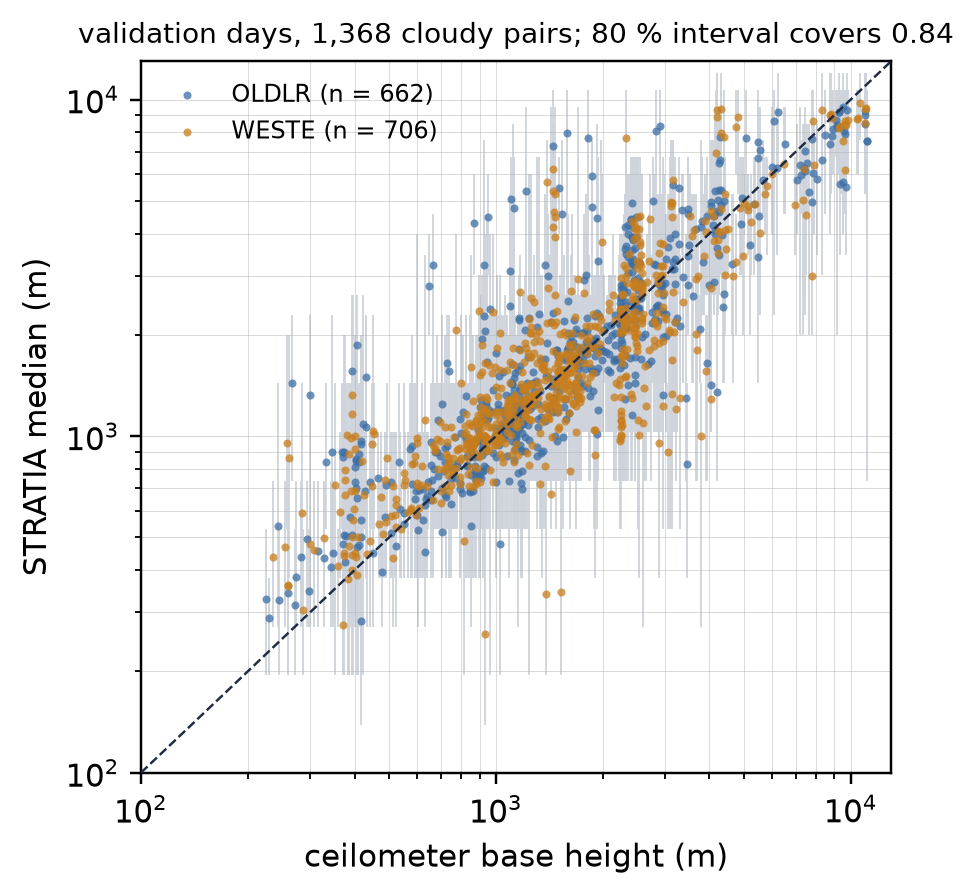
\includegraphics[width=\linewidth]{fig/cbh_scatter.png}
\caption{Predicted against ceilometer cloud-base height on the validation days (log axes), with the 80\,\%
conformal interval of each pair in grey.}
\label{fig:cbh}
\end{figure}

\subsection{Sky parse, OOD and glare}
The dense head reaches a sky/cloud/glare mIoU of \nSkyMiou{} on the pooled test masks and a layer mIoU of
\nLayerMiou{} on Almer\'ia; on the clear-sky test frames it still calls \nClearCloud{} of the pixels cloud, most of
it in the circumsolar region. The OOD score separates the owner's camera from the in-domain test frames at an
AUROC of \nOodAuroc{}. Under a synthetic Sun-glare corruption on validation, \'etage F1 drops from 0.838 to 0.760,
sky mIoU from 0.901 to 0.816, and the clear-sky cloud fraction rises from 0.29 to 0.47: glare is the single
failure mode we can name, and the parse rather than the recognition is what it breaks.

\subsection{Ablations}
\begin{table}[t]
\centering
\small
\begin{tabular}{llrr}
\toprule
Group & Variant & Étage F1 & Genus F1 \\
\midrule
reference & Gate G4 heads (geometry dropout 0.3, soft and set-valued targets, hier & 0.817 & 0.719 \\
geometry (SkyRay) & no geometry: ray map and Sun always dropped (p\_drop 1.0) & 0.809 & 0.720 \\
geometry (SkyRay) & geometry always given (p\_drop 0.0) & 0.829 & 0.709 \\
targets & hard targets: first listed genus, majority étages, majority okta & 0.794 & 0.729 \\
loss & no hierarchy loss (lambda\_h 0) & 0.813 & 0.712 \\
loss & uncertainty (Kendall) task weighting & 0.814 & 0.716 \\
Eye2Sky étage rows & without the ceilometer étage rows (indomain) & 0.823 & 0.738 \\
Eye2Sky étage rows (LODO) & held-out ccsn, with Eye2Sky étage rows & 0.489 & – \\
Eye2Sky étage rows (LODO) & held-out ccsn, without & 0.486 & – \\
Eye2Sky étage rows (LODO) & held-out mgcd, with Eye2Sky étage rows & 0.749 & – \\
Eye2Sky étage rows (LODO) & held-out mgcd, without & 0.871 & – \\
Eye2Sky étage rows (LODO) & held-out montenegro, with Eye2Sky étage rows & 0.360 & – \\
Eye2Sky étage rows (LODO) & held-out montenegro, without & 0.258 & – \\
Eye2Sky étage rows (LODO) & held-out almeria, with Eye2Sky étage rows & 0.593 & – \\
Eye2Sky étage rows (LODO) & held-out almeria, without & 0.327 & – \\
regularisation (P080) & head dropout 0 & 0.804 & 0.703 \\
regularisation (P080) & head dropout 0.3 & 0.817 & 0.743 \\
regularisation (P080) & weight decay 0 & 0.816 & 0.722 \\
regularisation (P080) & weight decay 0.2 & 0.815 & 0.715 \\
regularisation (P080) & no EMA & 0.820 & 0.711 \\
regularisation (P080) & EMA 0.999 & 0.812 & 0.708 \\
\bottomrule
\end{tabular}
\caption{Ablations of the global heads on validation data (one seed; the reference's three-seed spread is below 0.01): mean étage macro-F1 over the sources and mean genus macro-F1; the LODO rows give the held-out fold's étage F1.}
\label{tab:ablations}
\end{table}

\Cref{tab:ablations} varies the global heads one factor at a time on validation (one seed; the three reference
seeds spread by less than 0.01 in mean \'etage F1). Dropping the geometry always (\nAblNoGeo) or giving it always
(\nAblGeoAlways) brackets the reference (\nAblRef) within a point either way: SkyRay is cheap and does not hurt, but
on these sources the signal in the pixels dominates. Collapsing the set-valued and soft targets to one hard label
costs more (\nAblHard): the \emph{sets} are worth more than the geometry. Removing the hierarchy loss (\nAblNoH) and
uncertainty-weighting the tasks (\nAblKendall) are within noise of the reference. The weak \'etage rows derived
from the ceilometers are what make the all-sky folds transfer: without them the held-out Almer\'ia fold drops from
0.593 to 0.327 and Montenegro from 0.360 to 0.258, while MGCD, whose \'etages follow its seven sky types, gains;
the four-fold mean goes from 0.486 to the 0.548 of C1. Joint multi-task training and LoRA unfreezing of the last
blocks, tried in earlier stages, did not beat the staged cached-feature training that the released model uses
(layer mIoU 0.544 jointly against 0.559 staged); the released ablation tables report them.

\subsection{Efficiency}
\begin{table}[t]
\centering
\footnotesize
\begin{tabular}{lrr}
\toprule
Setting & Median ms & p95 ms \\
\midrule
PyTorch fp32, RTX 4050, batch 1 & 19.5 & 23.7 \\
PyTorch fp16, RTX 4050, batch 1 & 15.0 & 16.2 \\
PyTorch fp32, RTX 4050, batch 8 & 16.5 & 16.5 \\
ONNX Runtime CPU, batch 1 & 144.1 & 149.4 \\
desktop app, DirectML, RTX 4050, batch 1 & 29.2 & 33.0 \\
desktop app, ONNX Runtime CPU, batch 1 & 148.7 & 153.7 \\
Raspberry Pi 5 & – & – \\
\bottomrule
\end{tabular}
\caption{Latency per frame (median / p95 of repeated runs) of the deployed graph; 23.4 M parameters, 46 GFLOPs at 512 x 512.}
\label{tab:efficiency}
\end{table}

The exported graph has \nParamsM{}\,M parameters, of which \nHeadsParamsM{}\,M are above the frozen backbone, and
runs at \nGFlops{}\,GFLOPs for one 512$\times$512 frame (\cref{tab:efficiency}); inside the desktop application on a
laptop GPU through DirectML it takes \nLatencyDml{}\,ms per frame, and \nLatencyCpu{}\,ms on the CPU provider. The
Raspberry Pi 5 figure is left blank: the edge student is planned but not measured.

\subsection{A new camera from three afternoons}
\label{sec:b0268}
\begin{table}[t]
\centering
\small
\begin{tabular}{lrrrr}
\toprule
Model & Exact étage set & Oktas $\pm$1 & Top genus in set & OOD flagged \\
\midrule
zero-shot & 0.000 & 0.017 & 0.121 & 0.508 \\
adapted on three afternoons & 0.463 & 0.671 & 1.000 & 0.000 \\
rater vs rater (ceiling) & 0.911 & 0.771 & – & – \\
\bottomrule
\end{tabular}
\caption{The owner's camera (Arducam B0268), locked day 2026-10-20, 120 frames never used before the final evaluation; scored against each of the two annotators and averaged.}
\label{tab:b0268}
\end{table}

The released graph was pointed at the authors' own fisheye camera, a lens, exposure and horizon no training image
shares. Zero-shot (\cref{tab:b0268}) it is useless and says so: it agrees with the two annotators on
\nZsEtage{} of \'etage sets and \nZsOktas{} of cover within one okta on the locked fourth day, and flags \nZsOod{} of
the frames as out of distribution. Fine-tuning the global heads on the three earlier afternoons (273 frames, source
replay, regression guard) and re-exporting brings the agreement to \nAdEtage{} and \nAdOktas{}, with the top genus
inside the annotators' set on every frame and no frame flagged; the two annotators agree with each other on
0.911 and 0.771. The adapted graph is the one the application ships, and the fourth day was read once, after the
graph was frozen.

\section{Limitations}
\label{sec:limitations}

\paragraph{Two criteria failed.} The heads do not beat a linear probe on cross-dataset \'etage by the margin we
asked for, and the smaller backbone trails the ViT-L probe on in-domain genus. We chose ViT-S/16 for the laptop and
edge budget; the honest reading of \cref{tab:recognition} is that for recognition alone a probe on a larger frozen
backbone is as good, and that the heads earn their keep on the set-valued, dense and height tasks. The conformal
intervals fitted on spring weeks under-cover a summer test season; a deployment must refit the radii on recent
ceilometer data or report the wider raw intervals.

\paragraph{Geography and seasons.} The ceilometer pairs come from one camera network in one region over four
months; the recognition sets are web images and three sites. The owner's camera is the only tropical sky in the
corpus, and only through adaptation. Skill at a site never seen in training is evidence of transfer, not of
global validity.

\paragraph{Camera identity.} Dataset identity is linearly readable from the features at 99.7\,\% and remains so
after training; our protocol holds cameras out rather than pretending otherwise, and the OOD state exists because a
new camera \emph{will} be recognised as new. Zero-shot on such a camera is near zero; three afternoons of labels
were needed. The owner's camera also had only a declared zenith pointing when it was adapted and tested; a
Sun-track fit on its logged frames afterwards puts the optical axis about $13^\circ$ off the zenith and the frame
about $160^\circ$ rotated, with the declared pose $107^\circ$ off the Sun in the median. The geometry it fed the
model was therefore uninformative (geometry dropout makes that a valid input), and the adaptation numbers include
this; a checkerboard calibration and the fitted pose are the first things to do before the next adaptation.

\paragraph{Labels.} The mid \'etage is rare on four of five sources and is the one the model misses; glare breaks
the sky parse; the human ceiling comes from one five-rater set whose test portion is two blocks of days. The
Eye2Sky \'etage rows are weak labels derived from the ceilometer's lowest base.

\paragraph{Not measured.} The Raspberry Pi 5 edge student, INT8 quantisation and self-training over more days of
the owner's camera are planned and not reported; the table cells are left blank rather than estimated.

\section{Conclusion}
\label{sec:conclusion}

STRATIA reads genus, \'etage, cover, a sky parse and a calibrated cloud-base height from one sky picture, at expert
level on the two quantities experts agree on, with ceilometer-level height that transfers to an unseen station,
and with an explicit \emph{uncertain} answer on a camera it has not seen. The protocol around it matters as much
as the model: leakage-grouped and camera-held-out splits, set-valued WMO labels, a measured human ceiling,
pre-registered criteria and a test set read once with the reason logged. Two of those criteria failed, and the
paper reports them with the same intervals as the ones that held. The code, splits, data card, locked results
and the desktop application are released so that the next sky camera can be evaluated the same way.

{
    \small
    \bibliographystyle{ieeenat_fullname}
    \bibliography{main}
}

\end{document}
